\documentclass[11pt,a4paper]{article}

\usepackage[margin=2.5cm]{geometry}
\usepackage[T1]{fontenc}
\usepackage{newtxtext,newtxmath}
\usepackage{microtype}
\usepackage{amsmath}
\usepackage{booktabs}
\usepackage{graphicx}
\usepackage{caption}
\usepackage{subcaption}
\usepackage{enumitem}
\usepackage{titlesec}
\usepackage{cite}
\usepackage{xcolor}
\usepackage[hidelinks]{hyperref}

\titleformat{\section}{\centering\normalsize\scshape}{\thesection.}{0.5em}{}
\titlespacing*{\section}{0pt}{12pt}{5pt}
\renewcommand{\thesubsection}{\Alph{subsection}}
\titleformat{\subsection}{\normalsize\itshape}{\thesubsection.}{0.5em}{}
\titlespacing*{\subsection}{0pt}{6pt}{2pt}

\renewcommand{\thetable}{\Roman{table}}
\captionsetup[table]{name=TABLE, labelsep=newline, font={footnotesize,sc},
  justification=centering, skip=4pt}
\captionsetup[figure]{name=Fig., labelsep=period, font=footnotesize}
\captionsetup[subfigure]{font=footnotesize}

\setlist{itemsep=1pt, topsep=3pt, leftmargin=2.2em}
\renewcommand{\arraystretch}{1.1}

\graphicspath{
  {../outputs/runs/20260908T152939.777879Z-development-0f73422e-0d444a/}
  {../outputs/runs/20260908T165150.697815Z-backtest-509b876c-aa730c/}
  {../outputs/runs/20260910T133543.269946Z-held-out-dad36cad-632a5e/}
}

% Generated by `python -m src.report_tables` from the accepted runs.
% Do not edit by hand.
\newcommand{\AnomalyCandidates}{39}
\newcommand{\CleanRows}{59{,}861}
\newcommand{\DevAllBreakEven}{none}
\newcommand{\DevAllDrawdown}{\textminus{}65.31\%}
\newcommand{\DevAllGross}{\textminus{}25.58\%}
\newcommand{\DevAllHighCost}{\textminus{}70.70\%}
\newcommand{\DevAllHit}{53.6\%}
\newcommand{\DevAllHitRate}{44.6\%}
\newcommand{\DevAllInvested}{8.0\%}
\newcommand{\DevAllLowCost}{\textminus{}43.74\%}
\newcommand{\DevAllMean}{\textminus{}0.13\%}
\newcommand{\DevAllMedian}{0.11\%}
\newcommand{\DevAllN}{233}
\newcommand{\DevAllNet}{\textminus{}57.47\%}
\newcommand{\DevAllSharpe}{\textminus{}0.957}
\newcommand{\DevAllTopFiveShare}{13.1\%}
\newcommand{\DevAllTrades}{233}
\newcommand{\DevBootAllIncludeZero}{all}
\newcommand{\DevBuyHold}{486.25\%}
\newcommand{\DevCandidates}{387}
\newcommand{\DevCombinedBreakEven}{none}
\newcommand{\DevCombinedDrawdown}{\textminus{}10.52\%}
\newcommand{\DevCombinedEvents}{6}
\newcommand{\DevCombinedGross}{\textminus{}8.79\%}
\newcommand{\DevCombinedHighCost}{\textminus{}10.96\%}
\newcommand{\DevCombinedHit}{33.3\%}
\newcommand{\DevCombinedHitRate}{33.3\%}
\newcommand{\DevCombinedInvested}{0.2\%}
\newcommand{\DevCombinedLowCost}{\textminus{}9.45\%}
\newcommand{\DevCombinedMean}{\textminus{}1.53\%}
\newcommand{\DevCombinedMedian}{\textminus{}1.27\%}
\newcommand{\DevCombinedN}{6}
\newcommand{\DevCombinedNet}{\textminus{}10.10\%}
\newcommand{\DevCombinedSharpe}{\textminus{}0.697}
\newcommand{\DevCombinedTopFiveShare}{98.3\%}
\newcommand{\DevCombinedTrades}{6}
\newcommand{\DevDriftMean}{0.061\%}
\newcommand{\DevDriftMedian}{0.027\%}
\newcommand{\DevEvents}{235}
\newcommand{\DevFeatureHours}{15{,}323}
\newcommand{\DevHFiveAnyCI}{[0.17\%, 1.57\%]}
\newcommand{\DevHFiveAnyEst}{0.87\%}
\newcommand{\DevHFiveAnyN}{220}
\newcommand{\DevHFiveAnyP}{0.015}
\newcommand{\DevHFiveBoot}{[0.05\%, 0.85\%]}
\newcommand{\DevHFiveCI}{[\textminus{}0.20\%, 1.07\%]}
\newcommand{\DevHFiveEst}{0.44\%}
\newcommand{\DevHFiveN}{300}
\newcommand{\DevHFiveP}{0.178}
\newcommand{\DevHFourBoot}{[\textminus{}1.02\%, 1.69\%]}
\newcommand{\DevHFourCI}{[\textminus{}1.00\%, 1.55\%]}
\newcommand{\DevHFourEst}{0.28\%}
\newcommand{\DevHFourHolm}{1.000}
\newcommand{\DevHFourN}{158}
\newcommand{\DevHFourP}{0.335}
\newcommand{\DevHOneBoot}{[\textminus{}0.43\%, 0.17\%]}
\newcommand{\DevHOneCI}{[\textminus{}0.47\%, 0.21\%]}
\newcommand{\DevHOneEst}{\textminus{}0.13\%}
\newcommand{\DevHOneHolm}{1.000}
\newcommand{\DevHOneN}{233}
\newcommand{\DevHOneP}{0.768}
\newcommand{\DevHOneVariantsIncludeZero}{every}
\newcommand{\DevHThreeBoot}{[\textminus{}1.00\%, 1.18\%]}
\newcommand{\DevHThreeCI}{[\textminus{}1.89\%, 1.91\%]}
\newcommand{\DevHThreeEst}{0.01\%}
\newcommand{\DevHThreeHolm}{1.000}
\newcommand{\DevHThreeN}{158}
\newcommand{\DevHThreeP}{0.495}
\newcommand{\DevHTwoBoot}{[\textminus{}0.28\%, 1.39\%]}
\newcommand{\DevHTwoCI}{[\textminus{}0.42\%, 1.41\%]}
\newcommand{\DevHTwoEst}{0.49\%}
\newcommand{\DevHTwoHolm}{0.578}
\newcommand{\DevHTwoN}{233}
\newcommand{\DevHTwoP}{0.144}
\newcommand{\DevHours}{35{,}025}
\newcommand{\DevInteractionBoot}{[\textminus{}8.47\%, \textminus{}1.40\%]}
\newcommand{\DevInteractionCI}{[\textminus{}8.51\%, \textminus{}0.55\%]}
\newcommand{\DevInteractionEst}{\textminus{}4.53\%}
\newcommand{\DevInteractionN}{158}
\newcommand{\DevInteractionP}{0.026}
\newcommand{\DevLeaveEventHigh}{8.98\%}
\newcommand{\DevLeaveEventLow}{\textminus{}5.51\%}
\newcommand{\DevLeaveYearHigh}{11.89\%}
\newcommand{\DevLeaveYearLow}{\textminus{}8.49\%}
\newcommand{\DevLowBreakEven}{none}
\newcommand{\DevLowDrawdown}{\textminus{}12.61\%}
\newcommand{\DevLowEvents}{25}
\newcommand{\DevLowGross}{\textminus{}0.58\%}
\newcommand{\DevLowHighCost}{\textminus{}10.04\%}
\newcommand{\DevLowHit}{52.0\%}
\newcommand{\DevLowHitRate}{44.0\%}
\newcommand{\DevLowInvested}{0.9\%}
\newcommand{\DevLowLowCost}{\textminus{}3.52\%}
\newcommand{\DevLowMean}{\textminus{}0.02\%}
\newcommand{\DevLowMedian}{0.19\%}
\newcommand{\DevLowN}{25}
\newcommand{\DevLowNet}{\textminus{}6.37\%}
\newcommand{\DevLowSharpe}{\textminus{}0.302}
\newcommand{\DevLowTopFiveShare}{56.5\%}
\newcommand{\DevLowTrades}{25}
\newcommand{\DevOtherHit}{54.1\%}
\newcommand{\DevOtherMean}{\textminus{}0.18\%}
\newcommand{\DevOtherMedian}{0.10\%}
\newcommand{\DevOtherN}{133}
\newcommand{\DevPositiveEvents}{236}
\newcommand{\DevPositiveHit}{50.6\%}
\newcommand{\DevPositiveMean}{0.26\%}
\newcommand{\DevPositiveMeanCI}{[\textminus{}0.11\%, 0.63\%]}
\newcommand{\DevPositiveMedian}{0.05\%}
\newcommand{\DevPositiveN}{235}
\newcommand{\DevSampleHOneN}{233}
\newcommand{\DevSampleHThreeN}{158}
\newcommand{\DevShockHours}{25{,}979}
\newcommand{\DevSixCI}{[\textminus{}0.31\%, 0.19\%]}
\newcommand{\DevSixMean}{\textminus{}0.06\%}
\newcommand{\DevSixN}{235}
\newcommand{\DevStrictThresholdTrades}{20}
\newcommand{\DevTwentyFourCI}{[\textminus{}0.24\%, 0.65\%]}
\newcommand{\DevTwentyFourMean}{0.21\%}
\newcommand{\DevTwentyFourN}{233}
\newcommand{\DevUnavailableEvents}{77}
\newcommand{\DevWeekdayEvents}{200}
\newcommand{\DevWeekdayHit}{53.3\%}
\newcommand{\DevWeekdayMean}{\textminus{}0.20\%}
\newcommand{\DevWeekdayMedian}{0.10\%}
\newcommand{\DevWeekdayN}{199}
\newcommand{\DevWeekendBreakEven}{14.7 bp}
\newcommand{\DevWeekendCCCI}{[\textminus{}0.80\%, 1.64\%]}
\newcommand{\DevWeekendCCEst}{0.42\%}
\newcommand{\DevWeekendCCN}{158}
\newcommand{\DevWeekendCCP}{0.502}
\newcommand{\DevWeekendDrawdown}{\textminus{}14.34\%}
\newcommand{\DevWeekendEvents}{35}
\newcommand{\DevWeekendGross}{10.54\%}
\newcommand{\DevWeekendHighCost}{\textminus{}3.52\%}
\newcommand{\DevWeekendHit}{55.9\%}
\newcommand{\DevWeekendHitRate}{50.0\%}
\newcommand{\DevWeekendInvested}{1.2\%}
\newcommand{\DevWeekendLowCost}{6.12\%}
\newcommand{\DevWeekendMean}{0.29\%}
\newcommand{\DevWeekendMedian}{0.30\%}
\newcommand{\DevWeekendN}{34}
\newcommand{\DevWeekendNet}{1.88\%}
\newcommand{\DevWeekendPositiveVariants}{4}
\newcommand{\DevWeekendSharpe}{0.100}
\newcommand{\DevWeekendTopFiveShare}{42.6\%}
\newcommand{\DevWeekendTrades}{34}
\newcommand{\DevWeekendVariants}{7}
\newcommand{\DevWeekendYears}{4}
\newcommand{\DevWeekendYearsPositive}{2}
\newcommand{\DuplicateRows}{0}
\newcommand{\ExcludedRows}{8}
\newcommand{\HoAllBreakEven}{none}
\newcommand{\HoAllDrawdown}{\textminus{}57.10\%}
\newcommand{\HoAllGross}{\textminus{}19.37\%}
\newcommand{\HoAllHighCost}{\textminus{}66.70\%}
\newcommand{\HoAllHit}{50.2\%}
\newcommand{\HoAllHitRate}{48.4\%}
\newcommand{\HoAllInvested}{11.7\%}
\newcommand{\HoAllLowCost}{\textminus{}38.15\%}
\newcommand{\HoAllMean}{\textminus{}0.10\%}
\newcommand{\HoAllMedian}{0.04\%}
\newcommand{\HoAllN}{221}
\newcommand{\HoAllNet}{\textminus{}52.57\%}
\newcommand{\HoAllSharpe}{\textminus{}1.328}
\newcommand{\HoAllTopFiveShare}{11.7\%}
\newcommand{\HoAllTrades}{221}
\newcommand{\HoBootAllIncludeZero}{all}
\newcommand{\HoBuyHold}{48.37\%}
\newcommand{\HoCandidates}{384}
\newcommand{\HoCombinedBreakEven}{none}
\newcommand{\HoCombinedDrawdown}{\textminus{}11.86\%}
\newcommand{\HoCombinedEvents}{15}
\newcommand{\HoCombinedGross}{\textminus{}4.65\%}
\newcommand{\HoCombinedHighCost}{\textminus{}10.20\%}
\newcommand{\HoCombinedHit}{40.0\%}
\newcommand{\HoCombinedHitRate}{40.0\%}
\newcommand{\HoCombinedInvested}{0.8\%}
\newcommand{\HoCombinedLowCost}{\textminus{}6.35\%}
\newcommand{\HoCombinedMean}{\textminus{}0.32\%}
\newcommand{\HoCombinedMedian}{\textminus{}0.52\%}
\newcommand{\HoCombinedN}{15}
\newcommand{\HoCombinedNet}{\textminus{}8.02\%}
\newcommand{\HoCombinedSharpe}{\textminus{}0.586}
\newcommand{\HoCombinedTopFiveShare}{59.9\%}
\newcommand{\HoCombinedTrades}{15}
\newcommand{\HoDriftMean}{0.020\%}
\newcommand{\HoDriftMedian}{0.045\%}
\newcommand{\HoEvents}{222}
\newcommand{\HoFeatureHours}{22{,}632}
\newcommand{\HoHFiveAnyCI}{[\textminus{}0.18\%, 0.70\%]}
\newcommand{\HoHFiveAnyEst}{0.26\%}
\newcommand{\HoHFiveAnyN}{341}
\newcommand{\HoHFiveAnyP}{0.251}
\newcommand{\HoHFiveBoot}{[\textminus{}0.04\%, 0.65\%]}
\newcommand{\HoHFiveCI}{[\textminus{}0.13\%, 0.70\%]}
\newcommand{\HoHFiveEst}{0.29\%}
\newcommand{\HoHFiveN}{437}
\newcommand{\HoHFiveP}{0.173}
\newcommand{\HoHFourBoot}{[\textminus{}1.49\%, 0.68\%]}
\newcommand{\HoHFourCI}{[\textminus{}1.60\%, 0.79\%]}
\newcommand{\HoHFourEst}{\textminus{}0.40\%}
\newcommand{\HoHFourHolm}{1.000}
\newcommand{\HoHFourN}{221}
\newcommand{\HoHFourP}{0.746}
\newcommand{\HoHOneBoot}{[\textminus{}0.29\%, 0.11\%]}
\newcommand{\HoHOneCI}{[\textminus{}0.38\%, 0.19\%]}
\newcommand{\HoHOneEst}{\textminus{}0.10\%}
\newcommand{\HoHOneHolm}{1.000}
\newcommand{\HoHOneN}{221}
\newcommand{\HoHOneP}{0.749}
\newcommand{\HoHOneVariantsIncludeZero}{every}
\newcommand{\HoHThreeBoot}{[\textminus{}0.71\%, 1.61\%]}
\newcommand{\HoHThreeCI}{[\textminus{}1.00\%, 1.85\%]}
\newcommand{\HoHThreeEst}{0.42\%}
\newcommand{\HoHThreeHolm}{1.000}
\newcommand{\HoHThreeN}{221}
\newcommand{\HoHThreeP}{0.279}
\newcommand{\HoHTwoBoot}{[\textminus{}1.25\%, 0.91\%]}
\newcommand{\HoHTwoCI}{[\textminus{}1.27\%, 0.99\%]}
\newcommand{\HoHTwoEst}{\textminus{}0.14\%}
\newcommand{\HoHTwoHolm}{1.000}
\newcommand{\HoHTwoN}{221}
\newcommand{\HoHTwoP}{0.598}
\newcommand{\HoHours}{22{,}632}
\newcommand{\HoInteractionBoot}{[\textminus{}5.94\%, 1.35\%]}
\newcommand{\HoInteractionCI}{[\textminus{}5.37\%, \textminus{}0.02\%]}
\newcommand{\HoInteractionEst}{\textminus{}2.69\%}
\newcommand{\HoInteractionN}{221}
\newcommand{\HoInteractionP}{0.049}
\newcommand{\HoLeaveEventHigh}{\textminus{}2.89\%}
\newcommand{\HoLeaveEventLow}{\textminus{}15.17\%}
\newcommand{\HoLeaveYearHigh}{\textminus{}5.84\%}
\newcommand{\HoLeaveYearLow}{\textminus{}10.48\%}
\newcommand{\HoLowBreakEven}{2.1 bp}
\newcommand{\HoLowDrawdown}{\textminus{}19.14\%}
\newcommand{\HoLowEvents}{64}
\newcommand{\HoLowGross}{2.72\%}
\newcommand{\HoLowHighCost}{\textminus{}20.49\%}
\newcommand{\HoLowHit}{46.9\%}
\newcommand{\HoLowHitRate}{45.3\%}
\newcommand{\HoLowInvested}{3.4\%}
\newcommand{\HoLowLowCost}{\textminus{}4.88\%}
\newcommand{\HoLowMean}{0.04\%}
\newcommand{\HoLowMedian}{\textminus{}0.24\%}
\newcommand{\HoLowN}{64}
\newcommand{\HoLowNet}{\textminus{}11.91\%}
\newcommand{\HoLowSharpe}{\textminus{}0.497}
\newcommand{\HoLowTopFiveShare}{24.3\%}
\newcommand{\HoLowTrades}{64}
\newcommand{\HoOtherHit}{51.6\%}
\newcommand{\HoOtherMean}{\textminus{}0.15\%}
\newcommand{\HoOtherMedian}{0.21\%}
\newcommand{\HoOtherN}{157}
\newcommand{\HoPositiveEvents}{216}
\newcommand{\HoPositiveHit}{53.7\%}
\newcommand{\HoPositiveMean}{0.20\%}
\newcommand{\HoPositiveMeanCI}{[\textminus{}0.09\%, 0.49\%]}
\newcommand{\HoPositiveMedian}{0.15\%}
\newcommand{\HoPositiveN}{216}
\newcommand{\HoSampleHOneN}{221}
\newcommand{\HoSampleHThreeN}{221}
\newcommand{\HoShockHours}{22{,}632}
\newcommand{\HoSixCI}{[\textminus{}0.21\%, 0.22\%]}
\newcommand{\HoSixMean}{0.00\%}
\newcommand{\HoSixN}{222}
\newcommand{\HoStrictThresholdTrades}{16}
\newcommand{\HoTwentyFourCI}{[\textminus{}0.25\%, 0.50\%]}
\newcommand{\HoTwentyFourMean}{0.13\%}
\newcommand{\HoTwentyFourN}{221}
\newcommand{\HoUnavailableEvents}{0}
\newcommand{\HoWeekdayEvents}{195}
\newcommand{\HoWeekdayHit}{51.5\%}
\newcommand{\HoWeekdayMean}{\textminus{}0.08\%}
\newcommand{\HoWeekdayMedian}{0.17\%}
\newcommand{\HoWeekdayN}{194}
\newcommand{\HoWeekendBreakEven}{none}
\newcommand{\HoWeekendCCCI}{[\textminus{}1.27\%, 0.99\%]}
\newcommand{\HoWeekendCCEst}{\textminus{}0.14\%}
\newcommand{\HoWeekendCCN}{221}
\newcommand{\HoWeekendCCP}{0.804}
\newcommand{\HoWeekendDrawdown}{\textminus{}19.74\%}
\newcommand{\HoWeekendEvents}{27}
\newcommand{\HoWeekendGross}{\textminus{}5.83\%}
\newcommand{\HoWeekendHighCost}{\textminus{}15.47\%}
\newcommand{\HoWeekendHit}{40.7\%}
\newcommand{\HoWeekendHitRate}{40.7\%}
\newcommand{\HoWeekendInvested}{1.4\%}
\newcommand{\HoWeekendLowCost}{\textminus{}8.83\%}
\newcommand{\HoWeekendMean}{\textminus{}0.22\%}
\newcommand{\HoWeekendMedian}{\textminus{}0.32\%}
\newcommand{\HoWeekendN}{27}
\newcommand{\HoWeekendNet}{\textminus{}11.74\%}
\newcommand{\HoWeekendPositiveVariants}{2}
\newcommand{\HoWeekendSharpe}{\textminus{}0.435}
\newcommand{\HoWeekendTopFiveShare}{49.2\%}
\newcommand{\HoWeekendTrades}{27}
\newcommand{\HoWeekendVariants}{7}
\newcommand{\HoWeekendYears}{3}
\newcommand{\HoWeekendYearsPositive}{0}
\newcommand{\InvalidRows}{0}
\newcommand{\MissingHours}{43}
\newcommand{\ParsedRows}{59{,}869}
\newcommand{\Segments}{19}
\newcommand{\SourceFiles}{82}
\newcommand{\QualityRows}{%
Observed clean hours & 35{,}025 & 22{,}632 \\
Hours with a valid shock score & 25{,}979 & 22{,}632 \\
Hours with every feature & 15{,}323 & 22{,}632 \\
}
\newcommand{\EventRows}{%
Negative candidates ($z<-2.5$) & 387 & 384 \\
Accepted after the 24-hour cooldown & 235 & 222 \\
\quad weekend & 35 & 27 \\
\quad weekday & 200 & 195 \\
\quad low activity & 25 & 64 \\
\quad activity rank unavailable & 77 & 0 \\
\quad weekend and low activity & 6 & 15 \\
Complete 12-hour outcome (H1, H2) & 233 & 221 \\
Complete outcome and features (H3, H4) & 158 & 221 \\
Accepted positive events ($z>2.5$) & 236 & 216 \\
}
\newcommand{\KeyResultRows}{%
All shock & 233 & \textminus{}57.47\% & \textminus{}0.957 & \textminus{}65.31\% & 221 & \textminus{}52.57\% & \textminus{}1.328 & \textminus{}57.10\% \\
Weekend & 34 & 1.88\% & 0.100 & \textminus{}14.34\% & 27 & \textminus{}11.74\% & \textminus{}0.435 & \textminus{}19.74\% \\
Low activity & 25 & \textminus{}6.37\% & \textminus{}0.302 & \textminus{}12.61\% & 64 & \textminus{}11.91\% & \textminus{}0.497 & \textminus{}19.14\% \\
Combined & 6 & \textminus{}10.10\% & \textminus{}0.697 & \textminus{}10.52\% & 15 & \textminus{}8.02\% & \textminus{}0.586 & \textminus{}11.86\% \\
\midrule
BTC buy and hold & 1 & 486.25\% & n/r & n/r & 1 & 48.37\% & n/r & n/r \\
}
\newcommand{\CostRows}{%
Development & All shock & \textminus{}25.58\% & \textminus{}43.74\% & \textminus{}57.47\% & \textminus{}70.70\% & none \\
 & Weekend & 10.54\% & 6.12\% & 1.88\% & \textminus{}3.52\% & 14.7 bp \\
 & Low activity & \textminus{}0.58\% & \textminus{}3.52\% & \textminus{}6.37\% & \textminus{}10.04\% & none \\
 & Combined & \textminus{}8.79\% & \textminus{}9.45\% & \textminus{}10.10\% & \textminus{}10.96\% & none \\
\midrule
Held out & All shock & \textminus{}19.37\% & \textminus{}38.15\% & \textminus{}52.57\% & \textminus{}66.70\% & none \\
 & Weekend & \textminus{}5.83\% & \textminus{}8.83\% & \textminus{}11.74\% & \textminus{}15.47\% & none \\
 & Low activity & 2.72\% & \textminus{}4.88\% & \textminus{}11.91\% & \textminus{}20.49\% & 2.1 bp \\
 & Combined & \textminus{}4.65\% & \textminus{}6.35\% & \textminus{}8.02\% & \textminus{}10.20\% & none \\
}
\newcommand{\GroupRows}{%
All negative events & 233 & \textminus{}0.13\% & 0.11\% & 53.6\% & 221 & \textminus{}0.10\% & 0.04\% & 50.2\% \\
\quad weekend & 34 & 0.29\% & 0.30\% & 55.9\% & 27 & \textminus{}0.22\% & \textminus{}0.32\% & 40.7\% \\
\quad weekday & 199 & \textminus{}0.20\% & 0.10\% & 53.3\% & 194 & \textminus{}0.08\% & 0.17\% & 51.5\% \\
\quad low activity & 25 & \textminus{}0.02\% & 0.19\% & 52.0\% & 64 & 0.04\% & \textminus{}0.24\% & 46.9\% \\
\quad other activity & 133 & \textminus{}0.18\% & 0.10\% & 54.1\% & 157 & \textminus{}0.15\% & 0.21\% & 51.6\% \\
\quad weekend and low activity & 6 & \textminus{}1.53\% & \textminus{}1.27\% & 33.3\% & 15 & \textminus{}0.32\% & \textminus{}0.52\% & 40.0\% \\
Positive events & 235 & 0.26\% & 0.05\% & 50.6\% & 216 & 0.20\% & 0.15\% & 53.7\% \\
\midrule
Non-candidate hours (context only) & 25{,}463 & 0.061\% & 0.027\% &  & 22{,}237 & 0.020\% & 0.045\% &  \\
}
\newcommand{\HypothesisRows}{%
H1 & Mean return & 233 & \textminus{}0.13\% & [\textminus{}0.47\%, 0.21\%] & 1.000 & 221 & \textminus{}0.10\% & [\textminus{}0.38\%, 0.19\%] & 1.000 & No \\
H2 & Weekend & 233 & 0.49\% & [\textminus{}0.42\%, 1.41\%] & 0.578 & 221 & \textminus{}0.14\% & [\textminus{}1.27\%, 0.99\%] & 1.000 & No \\
H3 & Activity score & 158 & 0.01\% & [\textminus{}1.89\%, 1.91\%] & 1.000 & 221 & 0.42\% & [\textminus{}1.00\%, 1.85\%] & 1.000 & No \\
H4 & Weekend, controlled & 158 & 0.28\% & [\textminus{}1.00\%, 1.55\%] & 1.000 & 221 & \textminus{}0.40\% & [\textminus{}1.60\%, 0.79\%] & 1.000 & No \\
}
\newcommand{\InferenceDetailRows}{%
Development & H1 & 0.17\% & 0.768 & 1.000 & [\textminus{}0.43\%, 0.17\%] & 10000/10000/0/0 \\
Development & H2 & 0.46\% & 0.144 & 0.578 & [\textminus{}0.28\%, 1.39\%] & 10000/10000/0/0 \\
Development & H3 & 0.96\% & 0.495 & 1.000 & [\textminus{}1.00\%, 1.18\%] & 10000/10000/0/0 \\
Development & H4 & 0.65\% & 0.335 & 1.000 & [\textminus{}1.02\%, 1.69\%] & 10000/10000/0/0 \\
\midrule
Held out & H1 & 0.15\% & 0.749 & 1.000 & [\textminus{}0.29\%, 0.11\%] & 10000/10000/0/0 \\
Held out & H2 & 0.57\% & 0.598 & 1.000 & [\textminus{}1.25\%, 0.91\%] & 10000/10000/0/0 \\
Held out & H3 & 0.73\% & 0.279 & 1.000 & [\textminus{}0.71\%, 1.61\%] & 10000/10000/0/0 \\
Held out & H4 & 0.61\% & 0.746 & 1.000 & [\textminus{}1.49\%, 0.68\%] & 10000/10000/0/0 \\
}
\newcommand{\GroupComparisonRows}{%
Development & Weekend minus weekday & 34 & 199 & 0.49\% & [\textminus{}0.42\%, 1.41\%] & [\textminus{}0.28\%, 1.42\%] \\
Development & Low minus other activity & 25 & 133 & 0.16\% & [\textminus{}0.79\%, 1.10\%] & [\textminus{}0.75\%, 0.98\%] \\
Development & Combined minus remaining & 6 & 152 & \textminus{}1.43\% & [\textminus{}3.79\%, 0.93\%] & [\textminus{}4.11\%, \textminus{}0.04\%] \\
\midrule
Held out & Weekend minus weekday & 27 & 194 & \textminus{}0.14\% & [\textminus{}1.27\%, 0.99\%] & [\textminus{}1.26\%, 0.93\%] \\
Held out & Low minus other activity & 64 & 157 & 0.20\% & [\textminus{}0.37\%, 0.76\%] & [\textminus{}0.34\%, 0.75\%] \\
Held out & Combined minus remaining & 15 & 206 & \textminus{}0.24\% & [\textminus{}1.38\%, 0.91\%] & [\textminus{}1.63\%, 0.91\%] \\
}
\newcommand{\RobustnessRows}{%
Primary rule & 1.88\% & 34 & \textminus{}11.74\% & 27 \\
Shock threshold $-2.0$ & 7.97\% & 60 & \textminus{}7.85\% & 47 \\
Shock threshold $-3.0$ & 6.91\% & 20 & 1.38\% & 16 \\
Hold 6 hours & 2.99\% & 35 & \textminus{}6.80\% & 27 \\
Hold 24 hours & 16.25\% & 34 & \textminus{}5.40\% & 27 \\
Enter one hour later & \textminus{}7.13\% & 34 & \textminus{}8.58\% & 27 \\
Cooldown 12 hours & \textminus{}12.34\% & 41 & \textminus{}9.23\% & 30 \\
Cooldown 48 hours & \textminus{}2.51\% & 29 & 1.99\% & 24 \\
Signals inside the weekend & \textminus{}2.55\% & 20 & 0.63\% & 12 \\
Signals whose hold reaches Monday & 4.54\% & 14 & \textminus{}12.30\% & 15 \\
Leave one event out (range) & \textminus{}5.51\% to 8.98\% &  & \textminus{}15.17\% to \textminus{}2.89\% &  \\
Leave one year out (range) & \textminus{}8.49\% to 11.89\% &  & \textminus{}10.48\% to \textminus{}5.84\% &  \\
}


\newcommand{\StudentName}{Matteo Cannata}
\newcommand{\StudentEmail}{matteo.cannata26@imperial.ac.uk}
\newcommand{\SubmissionDate}{15 October 2026}

\begin{document}

\begin{center}

\includegraphics[width=4.8cm]{../logo/Imperial_College_London_new_logo.png}\par
\vspace{7pt}
{\normalsize\bfseries\StudentName\par}
\vspace{2pt}
{\footnotesize\SubmissionDate\par}
\vspace{10pt}
{\fontsize{17}{21}\selectfont\bfseries Buy the Weekend Dip?\par}
\vspace{3pt}
{\normalsize\bfseries Bitcoin Reversals After Extreme Sell-Offs\par}
\vspace{7pt}
{\small\href{mailto:\StudentEmail}{\StudentEmail}\par}
\vspace{8pt}
{\color{black}\rule{4.8cm}{0.4pt}\par}
\end{center}
\vspace{4pt}

\noindent{\small\bfseries\textit{Abstract}: Does Bitcoin rebound after an extreme one-hour sell-off, and is the rebound larger at weekends or when trading activity before the sell-off was low? This study tests both questions on hourly Binance BTCUSDT spot data. The primary rules and tests were fixed before outcomes were inspected; 2020 to 2023 was used for development, and January 2024 to July 2026 was held out for one primary historical evaluation. In both periods the average 12-hour log return after a negative shock was slightly negative (\DevAllMean{} and \HoAllMean{}), and none of H1 to H4 was supported held out. The all-shock rule returned \HoAllNet{} held out after assumed costs; the weekend rule, which gained \DevWeekendNet{} in development, returned \HoWeekendNet{} held out.\par}
\vspace{5pt}

\section{Hypothesis Pitch}\par

After an unusually large one-hour fall in BTCUSDT, I expect a partial recovery over the next 12 hours, with a larger rebound at weekends or after 24 hours of low trading activity. My central question is whether weekend timing adds information beyond the activity observed before the fall.

Temporary selling pressure could push prices down before easing, allowing a rebound. A fall driven by new information could instead continue. Lower preceding activity might accompany stronger temporary price pressure, but this is a proposed explanation: the hourly candles cannot identify its cause.

Previous evidence of short-term Bitcoin mean reversion and reversal after negative hourly shocks makes a rebound plausible~\cite{denicola,miralles}. Evidence of stronger daily reversal strategy returns across cryptocurrency pairs when volume is low relative to its recent trend motivates testing activity as well~\cite{bianchi}. These findings leave open whether pre-shock activity matters within BTCUSDT and whether weekend timing adds information beyond it.

In De Nicola's Bitstamp sample, weekend volume was about 20\% below the weekly average~\cite{denicola}, but that does not establish a weekend rebound. A quiet weekday could resemble a quiet weekend. I therefore compare weekend timing and activity separately, then ask whether the weekend association remains after adding activity and other controls. I measure activity using the USDT value traded before the shock. This records completed trading, but does not reveal the available orders, spreads or depth.

Four predictions were fixed before outcomes were inspected. I would set aside each unless the held-out data show:
\begin{enumerate}[label=\arabic*)]
\item a positive mean 12-hour return after negative shocks (H1);
\item a higher mean after weekend than weekday shocks (H2);
\item a higher return after lower pre-shock activity (H3);
\item a positive weekend association after controlling for activity, shock size, recent volatility and time of day (H4).
\end{enumerate}
Each needs the expected sign and a Holm-adjusted one-sided $p$-value below 0.05. An unsupported test does not establish that the effect is absent; all planned analyses continue. Secondary H5 compares positive and negative shocks. Separately, I would reject the trading case if development gains failed held out or disappeared after costs.

\newpage
\section{Data Pipeline}

Archives are downloaded and verified, cleaned and divided into contiguous segments. Past-only features identify shock candidates; chronological cooldown sets event acceptance. Counts and timestamp-only availability are audited before outcomes. Accepted negative events feed the event study and simulated trades. Development checks precede the freeze of rules and inputs and the held-out evaluation.

\subsection{Data Source and Snapshot}

The code downloads \SourceFiles{} official Binance BTCUSDT spot monthly archives~\cite{binance}, verifies each ZIP against Binance's published SHA-256 checksum and preserves it unchanged in \texttt{data/raw/}. Their hourly OHLC prices, volume and trade counts cover October 2019 to July 2026. The 6-, 12- and 24-hour analyses all use these one-hour candles. No credentials are needed.

\subsection{Sample Periods}

October to December 2019 warms up rolling features. Development covers 2020 to 2023; January 2024 to July 2026 is held out. Weekend and split labels use the unrounded UTC source close time.

\subsection{Cleaning and Missing Data}

Binance switched spot archive timestamps from milliseconds to microseconds on 1 January 2025~\cite{binance}. The parser enforces the expected unit, 12-column schema and numeric/OHLC consistency. Invalid values or duplicate/disordered timestamps stop validation; the snapshot contains none (Table~\ref{tab:quality}).

\ExcludedRows{} non-standard close-time rows coinciding with exchange interruptions are excluded. The cleaned grid has \MissingHours{} missing hours, including these exclusions: 4 in warm-up, 39 in development and none held out, forming \Segments{} contiguous segments. Manual raw-file checks retained all \AnomalyCandidates{} distinct rows identified by the 20 largest returns and 20 largest close-to-next-open gaps.

No candle is imputed. Gaps invalidate crossing returns and outcomes and restart rolling histories. Bitcoin needs no split or dividend adjustment.

\begin{table}[ht]
\centering\small
\caption{Data quality (left) and hours each calculation can use (right)}
\label{tab:quality}
\begin{tabular}[t]{@{}lr@{}}
\toprule
Raw archive, Oct 2019 to Jul 2026 & Rows \\
\midrule
Monthly files & \SourceFiles{} \\
Rows parsed & \ParsedRows{} \\
Excluded (non-standard close) & \ExcludedRows{} \\
Duplicate / invalid rows & \DuplicateRows{} / \InvalidRows{} \\
Clean rows & \CleanRows{} \\
Missing hours & \MissingHours{} \\
\bottomrule
\end{tabular}\hspace{2em}
\begin{tabular}[t]{@{}lrr@{}}
\toprule
 & Development & Held out \\
\midrule
\QualityRows
\bottomrule
\end{tabular}
\end{table}

\subsection{Shock Events and Features}

Features use information available at the shock close. The hourly log return is $r_t=\ln(C_t/C_{t-1})$, requiring a contiguous previous hour. The score $z_t=(r_t-\bar r)/s$ uses the mean $\bar r$ and sample standard deviation $s$ of the previous 720 returns (30 days), excluding $r_t$. A candle with $z_t<-2.5$ is a negative-shock candidate.

Candidates are processed chronologically: accept the first, then suppress same-sign candidates less than 24 hours after the last accepted event. This limits repeated signals from one sell-off. Future prices and outcomes never determine acceptance.

Pre-shock activity $A_t$ is the USDT quote volume of the previous 24 hours, excluding the shock hour. Its rank $P_t$ is the share of the previous 2,160 values of $A$ (90 days) less than or equal to it. Each reference value needs 24 prior hours, so the full rank requires 2,184 uninterrupted hours. Regressions use $1-P_t$; low activity means $P_t<1/3$. Quote volume measures activity, not liquidity.

Controls are shock size ($-z_t$), realised volatility of the previous 24 returns, and four six-hour UTC time-of-day blocks.

The outcome $\ln(C_{t+12}/C_t)$ is the 12-hour log return after the shock, available only when all 12 following hours are contiguous and within one split. Table~\ref{tab:events} reconciles counts audited before outcomes.

\begin{center}
\begin{minipage}{\linewidth}
\centering\small
\captionof{table}{Shock events at each step}
\label{tab:events}
\begin{tabular}{@{}lrr@{}}
\toprule
 & Development & Held out \\
\midrule
\EventRows
\bottomrule
\end{tabular}
\end{minipage}
\end{center}

Event acceptance and later eligibility are separate. Of the \DevEvents{} accepted development negative shocks, \DevSampleHOneN{} have complete 12-hour outcomes and \DevSampleHThreeN{} also have every controlled-regression covariate (Table~\ref{tab:events}). Missing features do not change accepted event identities. The all-shock and weekend strategies require valid execution bars; low-activity and combined strategies additionally require an activity rank.

\section{Strategy and Backtest}

\subsection{Key Results}

\begin{table}[ht]
\centering\small
\caption{Key results at the primary cost (10 bp fee and 2 bp slippage per side)}
\label{tab:key}
\setlength{\tabcolsep}{4pt}
\begin{tabular}{@{}lrrrrrrrr@{}}
\toprule
 & \multicolumn{4}{c}{Development, in-sample} & \multicolumn{4}{c}{Held out, out-of-sample} \\
\cmidrule(lr){2-5}\cmidrule(l){6-9}
Strategy & Trades & Net return & Sharpe & Max DD & Trades & Net return & Sharpe & Max DD \\
\midrule
\KeyResultRows
\bottomrule
\end{tabular}

\smallskip
\parbox{\linewidth}{\footnotesize Net return is the cumulative return after costs over the whole period. The Sharpe ratio uses daily returns, annualised with 365 days and a zero risk-free rate. The recorded daily series samples equity at midnight after any new entry, so a midnight entry cost is assigned to the preceding day. This boundary convention can slightly change Sharpe relative to a mark immediately before the new entry. Maximum drawdown (Max DD) is measured on the hourly equity curve. The held-out combined rule has \HoCombinedTrades{} trades; its annualised Sharpe is descriptive and highly unstable. Buy and hold has a different exposure and is not risk-matched; n/r means not reported.}
\end{table}

Table~\ref{tab:key} gives the required metrics. At the primary settings, all four strategies lost money held out after costs. The weekend rule, the main candidate, returned \DevWeekendNet{} in development (Sharpe \DevWeekendSharpe{}) and \HoWeekendNet{} out-of-sample (Sharpe \HoWeekendSharpe{}, maximum drawdown \HoWeekendDrawdown{}). Buying every shock returned \DevAllNet{} and \HoAllNet{}. Over the held-out period, simply holding Bitcoin returned \HoBuyHold{}.

\subsection{Trading Rules}

When a qualifying negative-shock candle closes, the rule buys BTC at the next hour's open and sells at the close 12 hours after the shock (entry $O_{t+1}$, exit $C_{t+12}$). Each trade invests 100\% of the account, without leverage, short selling or a stop-loss. One position is open at a time; otherwise the account holds USDT. Four separate accounts start at 1.0 and trade all shocks, weekend shocks, low-activity shocks, or shocks that are both. All four are reported. Missing entry-to-exit hours cancel the trade. Event-study log returns begin at the shock close; portfolio wealth compounds arithmetic net trade returns from next-open execution after costs.

\subsection{Transaction Costs}

Costs are charged on every fill. With fee $f$ and slippage $s$ per side, the buy price is $O(1+s)$, the sell price is $C(1-s)$, and each trade multiplies wealth by $(1-f)^2\,C(1-s)/\big(O(1+s)\big)$. The primary case assumes $f=10$~bp and $s=2$~bp, about 24~bp per round trip. A low case (5~bp fee, 1~bp slippage) and a high case (10~bp, 10~bp) were fixed in advance.

\subsection{Statistical Tests}

Each hypothesis is tested with an ordinary least-squares regression on shock events, separately by period. Model~0 estimates the mean outcome (H1). Model~1 adds a weekend indicator (H2). Model~2 adds the activity score, shock size, volatility and time-of-day controls, giving H3 (activity) and H4 (weekend after controls). Secondary Model~3 adds a weekend $\times$ activity interaction. HC3 standard errors account for unequal residual variance, but cannot rule out dependence between shocks. Holm's correction limits false positives across the four one-sided H1 to H4 tests. As a check on within-month dependence, a bootstrap resamples whole calendar months 10,000 times and refits each model.

\subsection{Returns After a Shock}

The rebound the hypothesis predicts does not appear on average. The mean 12-hour log return after a negative shock is \DevAllMean{} in development and \HoAllMean{} out-of-sample, against \DevDriftMean{} and \HoDriftMean{} for eligible non-candidate hours (Table~\ref{tab:groups}). Medians are slightly positive (\DevAllMedian{} and \HoAllMedian{}), so the negative means are pulled down by a tail of continued falls. The weekend group is positive in development (\DevWeekendMean{}, $N=\DevWeekendN$) but negative out-of-sample (\HoWeekendMean{}, $N=\HoWeekendN$). The average path (Fig.~\ref{fig:path}) is small and noisy; in both periods it is below zero at 12 hours and stays positive only from hour 19 in development and hour 18 out-of-sample.

\begin{table}[ht]
\centering\small
\caption{12-hour log return after shock events}
\label{tab:groups}
\setlength{\tabcolsep}{4pt}
\begin{tabular}{@{}lrrrrrrrr@{}}
\toprule
 & \multicolumn{4}{c}{Development} & \multicolumn{4}{c}{Held out} \\
\cmidrule(lr){2-5}\cmidrule(l){6-9}
Group & N & Mean & Median & Hit rate & N & Mean & Median & Hit rate \\
\midrule
\GroupRows
\bottomrule
\end{tabular}

\smallskip
\parbox{\linewidth}{\footnotesize Hit rate is the share of events with a positive 12-hour return. Non-candidate hours satisfy $z_t\ge-2.5$, including positive extremes; their windows overlap, so this row is context, not a formal comparison.}
\end{table}

The secondary event-study means are also uncertain. At 6 hours they are \DevSixMean{} ($N=\DevSixN$, HC3 95\% CI \DevSixCI{}) in development and \HoSixMean{} ($N=\HoSixN$, CI \HoSixCI{}) held out; at 24 hours they are \DevTwentyFourMean{} ($N=\DevTwentyFourN$, CI \DevTwentyFourCI{}) and \HoTwentyFourMean{} ($N=\HoTwentyFourN$, CI \HoTwentyFourCI{}).

The direct group comparisons in Table~\ref{tab:groupcomparisons} use indicator regressions with HC3 uncertainty and a calendar-month block bootstrap. The group medians and counts are in Table~\ref{tab:groups}; the combined group is sparse, especially in development ($N=\DevCombinedN$). Its development block interval excludes zero while the HC3 interval includes it, so that small-cell comparison is not a stable finding.

\begin{table}[ht]
\centering\footnotesize
\caption{12-hour group differences in mean log return}
\label{tab:groupcomparisons}
\setlength{\tabcolsep}{4pt}
\begin{tabular}{@{}llrrrcc@{}}
\toprule
Period & Difference & $N_1$ & $N_0$ & Estimate & HC3 95\% CI & Block 95\% CI \\
\midrule
\GroupComparisonRows
\bottomrule
\end{tabular}
\end{table}

\begin{figure}[ht]
\centering
\begin{subfigure}{0.49\textwidth}
  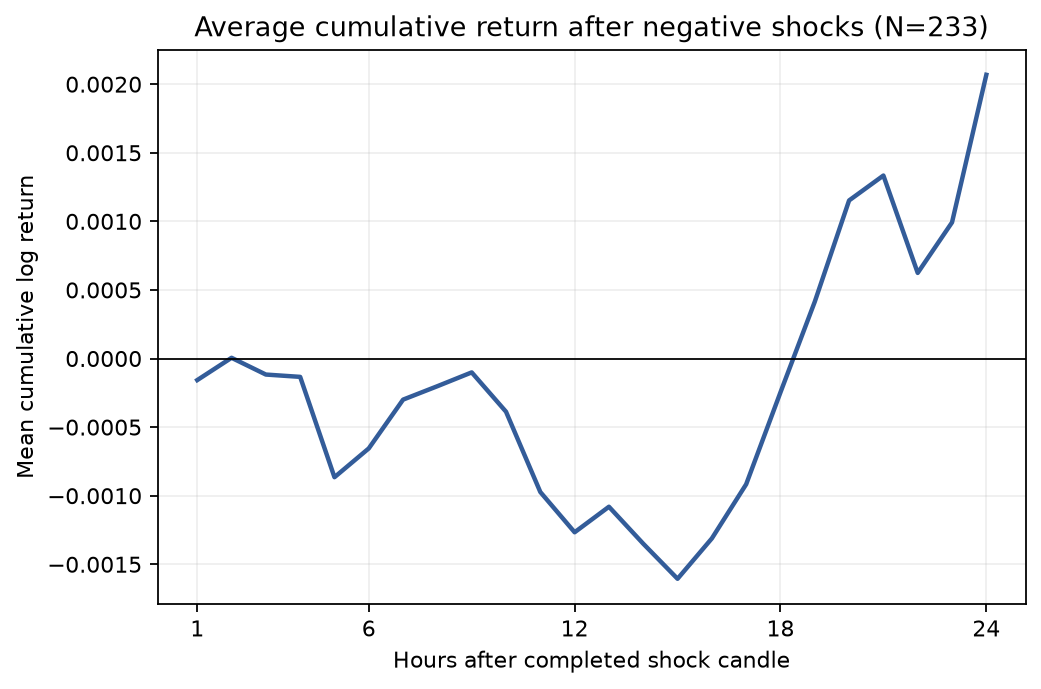
\includegraphics[width=\linewidth]{development_average_path.png}
  \caption{Development, $N=\DevAllN$}
\end{subfigure}\hfill
\begin{subfigure}{0.49\textwidth}
  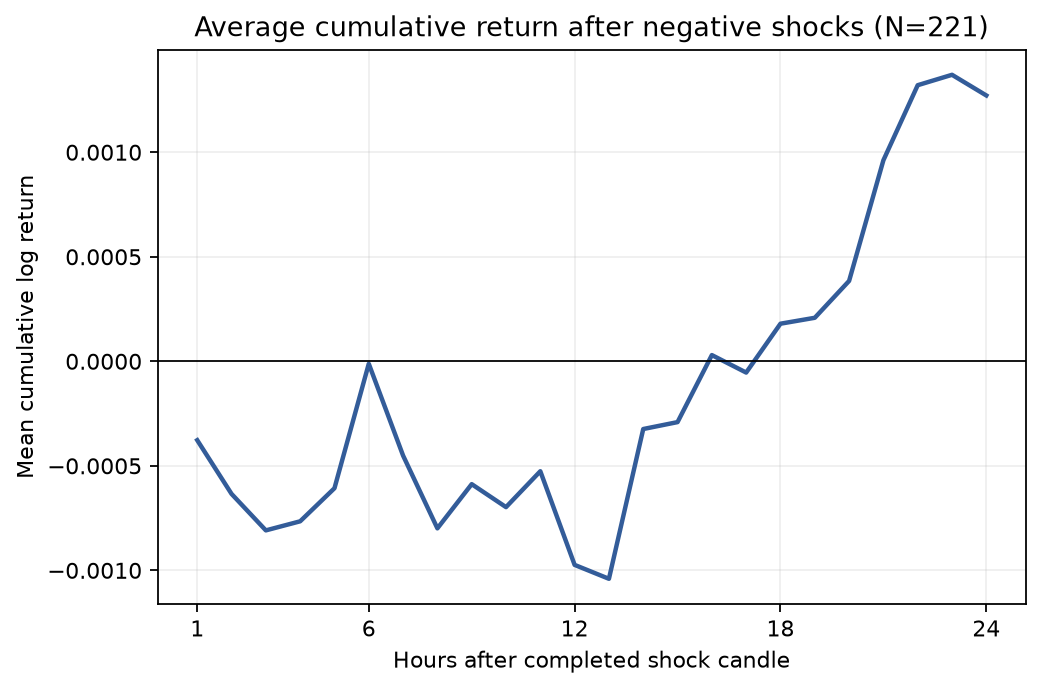
\includegraphics[width=\linewidth]{held_out_average_path.png}
  \caption{Held out, $N=\HoAllN$}
\end{subfigure}
\caption{Average cumulative log return in the 24 hours after a negative shock.}
\label{fig:path}
\end{figure}

\subsection{Hypothesis Test Results}

None of H1 to H4 is supported in the held-out period (Table~\ref{tab:hyp}). All four primary HC3 intervals include zero in both periods, as do their month-block bootstrap intervals. The two weekend estimates change sign between the periods. The weekend difference (H2) is \DevHTwoEst{} in development but \HoHTwoEst{} out-of-sample. After controls (H4), the development weekend coefficient falls slightly, from \DevWeekendCCEst{} to \DevHFourEst{} on the same events; out-of-sample it moves from \HoWeekendCCEst{} to \HoHFourEst{}. The activity coefficient (H3) is \DevHThreeEst{} and \HoHThreeEst{}, with intervals of \DevHThreeCI{} and \HoHThreeCI{}: too wide to show any reliable association.

\begin{table}[ht]
\centering\footnotesize
\caption{Main hypothesis tests}
\label{tab:hyp}
\setlength{\tabcolsep}{3pt}
\begin{tabular}{@{}llrrcrrrcrc@{}}
\toprule
 & & \multicolumn{4}{c}{Development} & \multicolumn{5}{c}{Held out} \\
\cmidrule(lr){3-6}\cmidrule(l){7-11}
 & Test & N & Estimate & 95\% CI & $p$ & N & Estimate & 95\% CI & $p$ & Supported \\
\midrule
\HypothesisRows
\bottomrule
\end{tabular}

\smallskip
\parbox{\linewidth}{\footnotesize H1 is the mean 12-hour log return (Model 0); H2 the weekend minus weekday difference (Model 1); H3 the activity score and H4 the weekend coefficient, both in Model 2. Intervals are two-sided 95\% HC3 intervals; $p$ is the Holm-adjusted one-sided value. Only the held-out columns decide support.}
\end{table}

Table~\ref{tab:inferencedetails} gives HC3 standard errors, raw one-sided $p$-values, block intervals and resample counts. HC3/Holm is primary; the bootstrap checks robustness.

\begin{table}[ht]
\centering\footnotesize
\caption{Additional inference details for H1 to H4}
\label{tab:inferencedetails}
\setlength{\tabcolsep}{4pt}
\begin{tabular}{@{}llrrrcc@{}}
\toprule
Period & Test & HC3 SE & Raw $p$ & Holm $p$ & Block 95\% CI & Draws A/V/E/R \\
\midrule
\InferenceDetailRows
\bottomrule
\end{tabular}

\smallskip
\parbox{\linewidth}{\footnotesize Draws A/V/E/R are attempted/valid/empty/rank-deficient month-block bootstrap replicates. The target is 10,000 valid draws per estimate, with at most 20,000 attempts. Standard errors and intervals use return-per-unit coefficients displayed as percentages.}
\end{table}

The secondary results lie outside the Holm family, use two-sided unadjusted tests, and are descriptive only. The Model~3 interaction is negative in both periods: \DevInteractionEst{} in development (HC3 95\% CI \DevInteractionCI{}, block CI \DevInteractionBoot{}, $p=\DevInteractionP$), based on only \DevCombinedN{} weekend low-activity events, and \HoInteractionEst{} out-of-sample (HC3 CI \HoInteractionCI{}, block CI \HoInteractionBoot{}, $p=\HoInteractionP$). The held-out HC3 interval barely excludes zero, while its block interval includes zero; this pattern is uncertain and requires a new pre-specified test.

H5 compares 12-hour returns after positive and negative shocks. The positive-minus-negative coefficient, conditional on absolute standardised shock size and the other specified covariates, is \DevHFiveEst{} in development (HC3 CI \DevHFiveCI{}, block CI \DevHFiveBoot{}, $p=\DevHFiveP$) and \HoHFiveEst{} held out (HC3 CI \HoHFiveCI{}, block CI \HoHFiveBoot{}, $p=\HoHFiveP$). The development HC3 and block intervals disagree about zero; held-out evidence does not establish asymmetry. With one cooldown shared by both signs, the coefficient is positive in both periods (\DevHFiveAnyEst{}, $p=\DevHFiveAnyP$ in development; \HoHFiveAnyEst{}, $p=\HoHFiveAnyP$ held out), but statistically distinguishable from zero only in development.

\subsection{Backtest and Cost Sensitivity}

Most rules lose before costs, and costs reduce every strategy's return (Table~\ref{tab:costs}, Fig.~\ref{fig:equity}).

\begin{center}
\begin{minipage}{\linewidth}
\centering\small
\captionof{table}{Cumulative return before costs and under each cost case}
\label{tab:costs}
\begin{tabular}{@{}llrrrrr@{}}
\toprule
Period & Strategy & Gross & Low cost & Primary & High cost & Break-even \\
\midrule
\CostRows
\bottomrule
\end{tabular}

\smallskip
\parbox{\linewidth}{\footnotesize Break-even is the cost per side at which the strategy ends where it started; ``none'' means it loses even at zero cost.}
\end{minipage}
\end{center}

Held-out all-shock return falls from \HoAllGross{} gross to \HoAllNet{} net. The development weekend rule breaks even at \DevWeekendBreakEven{} per side, while the only held-out rule positive gross, low activity (\HoLowGross{}), breaks even at \HoLowBreakEven{}.

\begin{figure}[ht]
\centering
\begin{subfigure}{0.49\textwidth}
  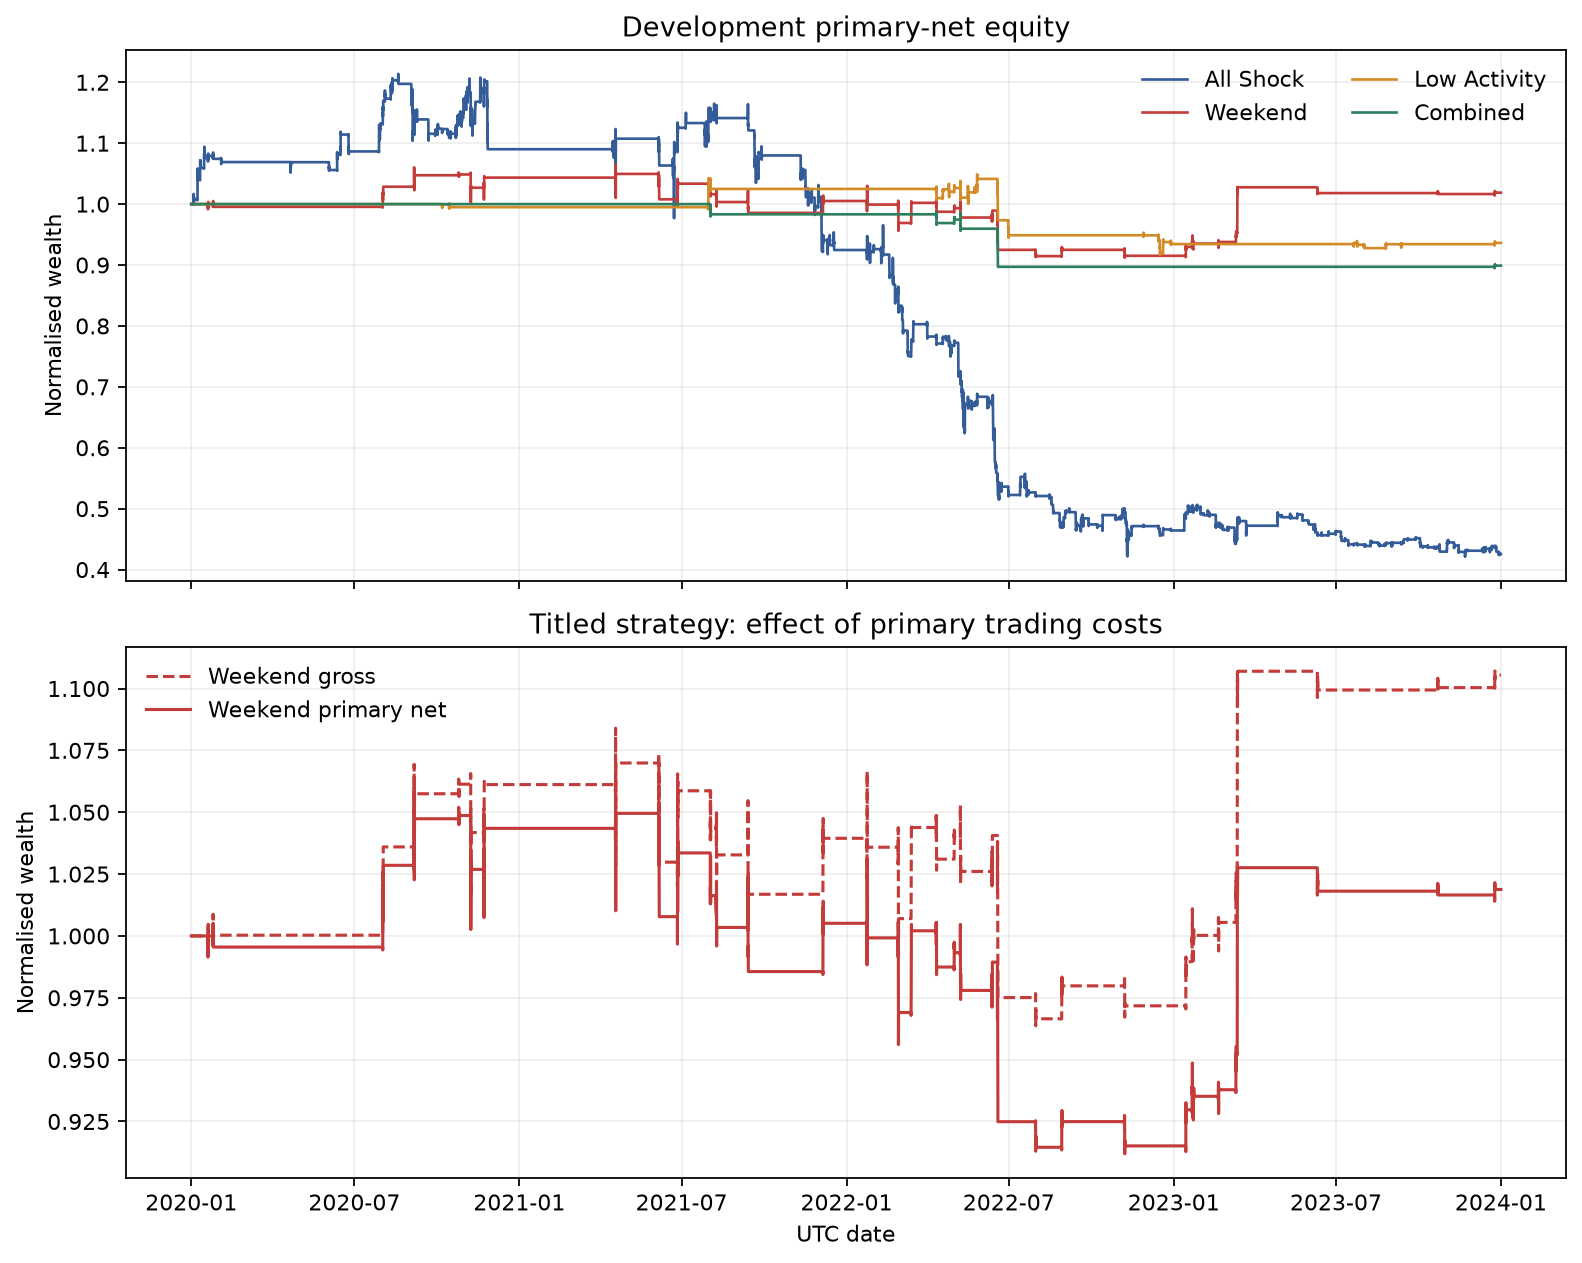
\includegraphics[width=\linewidth]{development_equity_curves.png}
  \caption{Development}
\end{subfigure}\hfill
\begin{subfigure}{0.49\textwidth}
  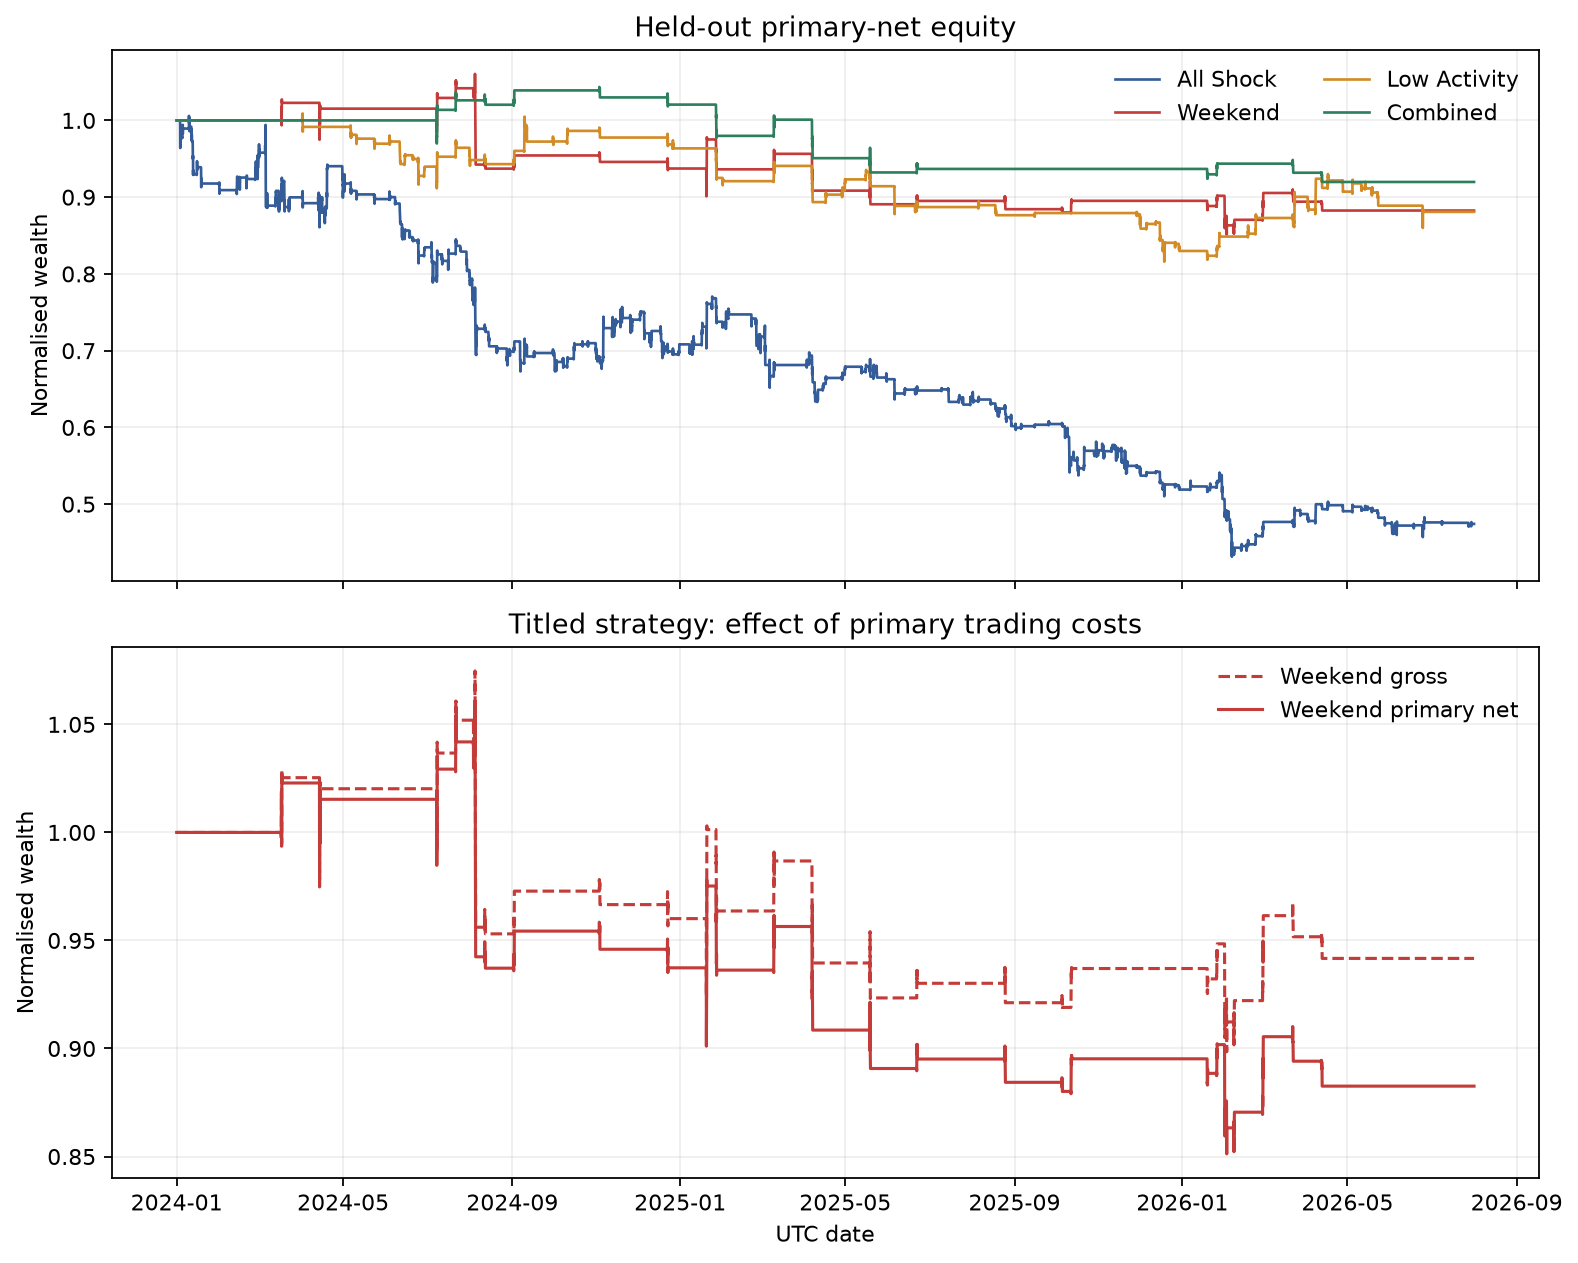
\includegraphics[width=\linewidth]{held_out_equity_curves.png}
  \caption{Held out}
\end{subfigure}
\caption{Net equity of the four rules at the primary cost (top panels), and the weekend rule before and after costs (bottom panels).}
\label{fig:equity}
\end{figure}

\subsection{Robustness Checks}

Each robustness check was fixed in advance and changes one setting at a time (Table~\ref{tab:robust}). In development, \DevWeekendPositiveVariants{} of the \DevWeekendVariants{} threshold, horizon, delay and cooldown variants of the weekend rule are positive, but the sign flips with a one-hour entry delay or a different cooldown, and removing a single event moves the result anywhere from \DevLeaveEventLow{} to \DevLeaveEventHigh{}. Out-of-sample, \HoWeekendPositiveVariants{} of the \HoWeekendVariants{} variants are positive: the $-3.0$ threshold, with only \HoStrictThresholdTrades{} trades, and the 48-hour cooldown. The rule loses money in each of the \HoWeekendYears{} held-out calendar years, and removing any single event still leaves it between \HoLeaveEventLow{} and \HoLeaveEventHigh{}. For H1, the confidence interval includes zero under every threshold, horizon and cooldown in both periods.

\begin{center}
\begin{minipage}{\linewidth}
\centering\small
\captionof{table}{Weekend rule when one setting is changed (net return at the primary cost)}
\label{tab:robust}
\begin{tabular}{@{}lrrrr@{}}
\toprule
 & \multicolumn{2}{c}{Development} & \multicolumn{2}{c}{Held out} \\
\cmidrule(lr){2-3}\cmidrule(l){4-5}
Setting & Net return & Trades & Net return & Trades \\
\midrule
\RobustnessRows
\bottomrule
\end{tabular}
\end{minipage}
\end{center}

\subsection{Interpretation}

I take three lessons from the results. First, there is no reliable positive mean return at the fixed 12-hour horizon in this Binance sample. Earlier reversal studies used different venues, periods and event definitions, so this does not directly refute them. Second, the development weekend gain was fragile: it rested on \DevWeekendTrades{} trades, its five largest trades made up \DevWeekendTopFiveShare{} of total absolute profit and loss, and its sign changed with the cooldown or entry time. The held-out loss confirms that this gain did not persist. Third, at about 24~bp per round trip, the assumed costs leave little room for a small rebound to become a net trading gain.

\section{Methodology Defense}

\subsection{Universe}

I chose BTCUSDT because it trades through weekends and Binance provides a public, checksummed history. Hourly candles define a signal from a completed bar and entry at the next open; they do not establish actual fills. This tests one surviving pair on one exchange, so findings may differ for other coins or venues.

\subsection{Train/Test Split}

I used 2020 to 2023 to develop the rule and kept the next 31 months, with \HoSampleHOneN{} usable shocks, for evaluation. A random split would mix nearby shocks and let later market conditions influence choices made for earlier ones. The chronological split asks whether the same rule survives a later period. If the market changed after 2023, that limits how far the development result carries forward.

\subsection{Signal Construction}

A fixed price-drop cut would flag many hours in volatile years and few in calm years. I instead scale each return by the previous 30 days, so the $-2.5$ threshold describes an unusual move relative to recent conditions; it yields \DevEvents{} development and \HoEvents{} held-out events. I fixed 2.5 before inspecting outcomes as a convention for relative extremeness, with 2.0 and 3.0 as sensitivity checks. The cutoff is not claimed to be optimal. The 24-hour cooldown keeps the first candidate from a sell-off. Counting every extreme hour would treat one episode as several events, while choosing the largest would require later prices. I chose 12 hours as a short window in which temporary pressure might fade, with 6 and 24 hours fixed as checks.

\subsection{Transaction Cost Assumptions}

Next-open fills follow the completed shock and remain a simulation assumption. The 10~bp fee is fixed; 2~bp slippage allows for spread and delay without order-book estimates. Higher costs worsen every return, and a one-hour delay reverses the development weekend gain (Table~\ref{tab:robust}).

\subsection{Activity Measure}

I use prior 24-hour USDT quote volume to summarise a full day before the shock. Ranking against 90 days provides a longer recent benchmark and adjusts for changing volume levels. H3 uses the continuous score $1-P_t$; the pre-set $P_t<1/3$ cutoff defines descriptive groups and trading filters. Trade count is an alternative check. Neither proxy measures order-book depth; high volume can accompany poor liquidity.

\subsection{Statistical Inference}

I refit the weekend-only model on Model~2's complete-case events, fixing sample composition when adding activity and controls. HC3 allows unequal residual variance; Holm guards H1 to H4 against chance findings. Month-block resampling probes within-month dependence; longer dependence may still leave intervals too narrow. Unmeasured news can affect shocks and subsequent returns, so coefficients describe associations, not causes.

\subsection{Limitations}

Sparse groups (\DevCombinedEvents{} and \HoCombinedEvents{} weekend low-activity events), a few influential shocks, missing order-book data, and unmodelled Binance and USDT risks limit inference and execution claims.

\section{Pitfall Checklist}

\subsection{Look-ahead bias}

I checked features, events and trades separately. Changing later observations leaves earlier shock, activity and volatility inputs unchanged. Rolling histories exclude the shock return and volume; future outcomes cannot change cooldown decisions. Tests verify next-open entry after a completed shock, exact exits, gap rejection, unrounded calendar labels and split-contained outcomes. No future prices or returns enter signal construction. Trades crossing missing-data gaps are excluded retrospectively for evaluability, which limits the backtest's realism.

\subsection{Survivorship bias}

There is no retrospectively filtered asset universe: the study preselects one pair. Bitcoin and Binance nevertheless survived while other coins and venues failed. A collapsing coin might have more permanent sell-offs, so the result cannot be generalised to all crypto assets.

\subsection{Overfitting/data-snooping}

One primary setting, four trading rules and 12 robustness and diagnostic families were fixed before outcomes. No grid search or post-result tuning was used; corrections are logged. Holm adjusts H1 to H4 for multiple testing. Every frozen variant was run. The \DevWeekendNet{} development weekend gain failed held out.

\subsection{Transaction costs and slippage}

The assumed costs are 10~bp fees and 2~bp slippage per side. Low and high cases and delayed entry test sensitivity; market impact is unmodelled. Held-out all-shock return falls from \HoAllGross{} gross to \HoAllNet{} net. In that period, only the low-activity rule is positive before costs, breaking even at \HoLowBreakEven{} per side; all four primary rules lose net.

\subsection{Out-of-sample validation}

Development used 2020 to 2023; January 2024 to July 2026 was held out. Before access, an outcome-free audit flagged sparse cells and code, configuration, inputs and development results were frozen. One primary evaluation was accepted. Weekend return fell from \DevWeekendNet{} (Sharpe \DevWeekendSharpe{}) to \HoWeekendNet{} (Sharpe \HoWeekendSharpe{}). This is historical pseudo-out-of-sample evidence, not live performance.

\section{Efficiency Touchpoint}

The notebook benchmark identifies month-block regression bootstrapping as the bottleneck: ten development estimates required 100,000 refits and about 20 seconds ($N\le300$, $k\le9$), versus 4 seconds for features. Each draw samples whole months, rebuilds inputs and refits. For $S$ estimates, $B$ draws, $N$ events and $k$ regressors, time is about $O(SBNk^2)$; working memory per bootstrap is $O(Nk+B)$ for inputs and coefficient draws. Building each model matrix once and resampling its rows could reduce repeated work. The current run is practical and reproducible.

\section{Risk Touchpoint}

The account takes one unleveraged BTC position at a time, using 100\% of capital and holding USDT between trades. It remains concentrated in BTC, Binance and USDT. Held-out weekend exposure is \HoWeekendInvested{} of the time, yet maximum drawdown is \HoWeekendDrawdown{}; brief exposure does not ensure small losses. Five trades account for \HoWeekendTopFiveShare{} of absolute profit and loss. Lasting negative information could sustain a decline throughout the 12-hour hold while spreads widen. With no stop-loss, the account bears that decline. Full-capital sizing is a research convention.

\section{Reflection}

Cleaning was harder than the statistical tests: interruptions, a timestamp-unit switch and irregular closes needed explicit handling. Requiring complete covariates reduced the development sample from \DevSampleHOneN{} outcome-eligible shocks to \DevSampleHThreeN{} controlled-model events. The reproducible pipeline, validation checks and frozen rules made the findings auditable.

I expected a positive 12-hour mean, but the development and held-out means were slightly negative. The low-activity weekend idea was unsupported; its exploratory interaction pointed the other way, with uncertain held-out robustness. I learned how convincing a \DevWeekendTrades{}-trade gain could look when a few trades drove it, and underestimated the effect of a 24~bp round trip. A plausible explanation and development profit must survive uncertainty, later data and costs before I can trust a rule.

Next I would pre-register the unchanged rules on other pairs and exchanges, and test whether order-book depth explains activity associations. This rule showed no held-out net edge under the assumed costs.

\begingroup
\renewcommand{\section}[2]{\begin{center}\normalsize\scshape References\end{center}}
\footnotesize
\begin{thebibliography}{4}
\setlength{\itemsep}{2pt}

\bibitem{denicola}
G.~De~Nicola, ``On the intraday behavior of Bitcoin,'' \emph{Ledger}, vol.~6, pp.~58 to 80, 2021, doi: \href{https://doi.org/10.5195/ledger.2021.213}{10.5195/ledger.2021.213}.

\bibitem{miralles}
J.~L.~Miralles-Quir\'os and M.~M.~Miralles-Quir\'os, ``Intraday Bitcoin price shocks: when bad news is good news,'' \emph{J. Appl. Econ.}, vol.~25, no.~1, pp.~1294 to 1313, 2022, doi: \href{https://doi.org/10.1080/15140326.2022.2151253}{10.1080/15140326.2022.2151253}.

\bibitem{bianchi}
D.~Bianchi, M.~Babiak, and A.~Dickerson, ``Trading volume and liquidity provision in cryptocurrency markets,'' \emph{J. Bank. Finance}, vol.~142, Art.~no.~106547, 2022, doi: \href{https://doi.org/10.1016/j.jbankfin.2022.106547}{10.1016/j.jbankfin.2022.106547}.

\bibitem{binance}
Binance, ``Binance Public Data,'' \href{https://github.com/binance/binance-public-data}{documentation}; BTCUSDT one-hour spot monthly archive: \url{https://data.binance.vision/?prefix=data/spot/monthly/klines/BTCUSDT/1h/}.

\end{thebibliography}
\endgroup

\end{document}
